%%%%%%%%%%%%%%%%%%%%%%%%%%%%%%%%%%%%%%%%%%%%%%%%%%%%%
%                                                   %
%     Penn State Colloquium Poster Template         %
%                                                   %
% Uses Penn State Colloquium class, with options:   %
%                                                   %
% Orientation:                                      %
%     portrait (default), landscape                 %
%                                                   %
% Paper size:                                       %
%     a4paper (default), a0paper, a1paper, a2paper, %
%     a3paper, a5paper, a6paper                     %
%%%%%%%%%%%%%%%%%%%%%%%%%%%%%%%%%%%%%%%%%%%%%%%%%%%%%
\documentclass{../psuposter}
\renewcommand{\templateimagepath}{../} 


%%%%%%%%%%%%%%%%%%%%%%%%%%%%%%%%%%%%%%%%%%%%%%%%%%%%%
%               Package Dependencies                %
%%%%%%%%%%%%%%%%%%%%%%%%%%%%%%%%%%%%%%%%%%%%%%%%%%%%%
\usepackage{natbib}
\usepackage{lipsum}                                % Dummy text
\usepackage[figwidth = 0.98\linewidth]{todonotes}  % Dummy image (and more!)
\usepackage[absolute, overlay]{textpos}            % Figure placement
\usepackage{braket}
\setlength{\TPHorizModule}{\paperwidth}
\setlength{\TPVertModule}{\paperheight}
\setcitestyle{numbers,square}


%%%%%%%%%%%%%%%%%%%%%%%%%%%%%%%%%%%%%%%%%%%%%%%%%%%%%
%                 AUTHOR AND TITLE                  %
%%%%%%%%%%%%%%%%%%%%%%%%%%%%%%%%%%%%%%%%%%%%%%%%%%%%%
\title{Black Holes and the Quantum Information Paradox}
\author{Andrew Strominger}
\institute{Center for the Fundamental Laws of Nature, Harvard University}


%%%%%%%%%%%%%%%%%%%%%%%%%%%%%%%%%%%%%%%%%%%%%%%%%%%%%
%                  BEGIN DOCUMENT                   %
%%%%%%%%%%%%%%%%%%%%%%%%%%%%%%%%%%%%%%%%%%%%%%%%%%%%%
\begin{document}
\begin{frame}
\begin{columns}[t, totalwidth=\textwidth]
\begin{column}{0.45\textwidth - 1cm}


%%%%%%%%%%%%%%%%%%%%%%%%%%%%%%%%%%%%%%%%%%%%%%%%%%%%%
%                 BLOCK: BIOGRAPHY                  %
%%%%%%%%%%%%%%%%%%%%%%%%%%%%%%%%%%%%%%%%%%%%%%%%%%%%%
    \begin{block}{Speaker Biographic Summary}
    	\begin{center}
    		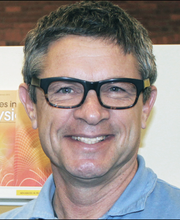
\includegraphics[width=0.6\textwidth]{images/strominger}
    	\end{center}
    	\href{https://www.physics.harvard.edu/people/facpages/strominger}{Dr. Andrew Strominger}, the Gwill E. York Professor of Physics at Harvard University, is a theoretical physicist renowned for his frontier work on quantum gravity and string theory.  He has received several honors, including the Physics Frontiers Breakthrough Prize, the Klein Medal from the Royal Swedish Academy of Sciences, the Dirac Medal from the Abdus Salam International Centre for Theoretical Physics, the Dannie Heineman Prize for Mathematical Physics of the American Physical Society, and a Guggenheim Fellowship. He is a Fellow of the American Physical Society and the American Association for the Advancement of Sciences and Member of the National Academy of Sciences and the American Academy of Arts and Sciences.
    \end{block}


%%%%%%%%%%%%%%%%%%%%%%%%%%%%%%%%%%%%%%%%%%%%%%%%%%%%%
%            BLOCK: RESEARCH INTERESTS              %
%%%%%%%%%%%%%%%%%%%%%%%%%%%%%%%%%%%%%%%%%%%%%%%%%%%%%
    \begin{block}{Research Interests}
        Prof. Strominger has made numerous, significant contributions to both quantum gravity and string theory. From discovering a string-theoretic origin of black hole entropy to uncovering an exact mathematical equivalence between QFT soft theorems, asymptotic symmetries, and the memory effect, Prof. Strominger's research efforts find exact mathematical equivalences in unique places.
        \begin{center}
	    	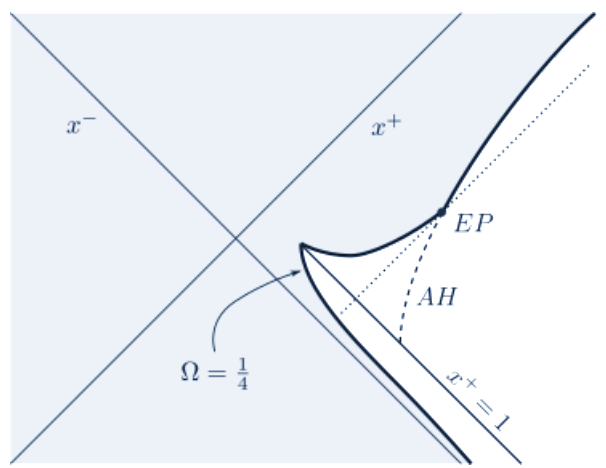
\includegraphics[width=0.55\textwidth]{images/kruskal}    		
    	\end{center}
    	\textit{Evaporating black hole in Kruskal coordinates}. \cite{hartmanIslandsAsymptoticallyFlat2020}
    \end{block}
\end{column}
\begin{column}{0.55\textwidth - 1cm}


%%%%%%%%%%%%%%%%%%%%%%%%%%%%%%%%%%%%%%%%%%%%%%%%%%%%%
%                 BLOCK: ABSTRACT                   %
%%%%%%%%%%%%%%%%%%%%%%%%%%%%%%%%%%%%%%%%%%%%%%%%%%%%%
    \begin{block}{Talk Abstract}
        The visible universe has edges, known as horizons, which surround black holes and other inaccessible spacetime regions. They are governed by a universal but still-mysterious set of laws discovered a half century ago by Stephen Hawking. These laws tell us that black holes are paradoxically both the simplest and most complex objects into the universe. The resolution of this paradox is a central goal of modern physics. Compelling progress in and future prospects for our understanding of black holes both from string theory and from the recent Event Horizon Telescope image will be described. 
    \end{block}


%%%%%%%%%%%%%%%%%%%%%%%%%%%%%%%%%%%%%%%%%%%%%%%%%%%%%
%                BLOCK: BACKGROUND                  %
%%%%%%%%%%%%%%%%%%%%%%%%%%%%%%%%%%%%%%%%%%%%%%%%%%%%%
    \begin{block}{Brief Background}
        The principle of conservation of information in quantum mechanics relates the state of a system at some time $\ket{\psi(t_0)}$ with the state at a later time $\ket{\psi(t>t_0)}$ via axiomatically chosen unitary operators. Consequently, for an isolated system, the total information must be conserved. Mathematically, the measure of the information in a system at any point in its evolution is captured by the Von Neumann entropy, which is analogous to the Shannon entropy from information theory. \cite{stromingerBlackHoleInformation2019}		
        \begin{center}
		   	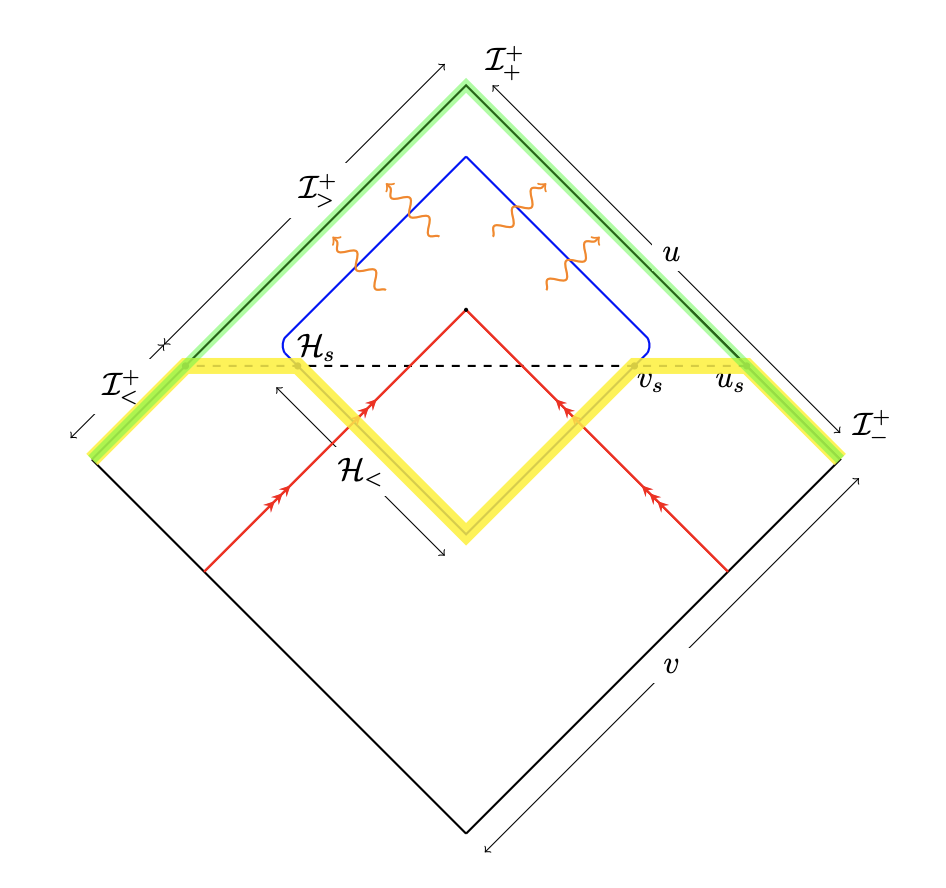
\includegraphics[width=0.45\textwidth]{images/evap}    		
    	\end{center}
		Classically, if an object falls into a blackhole, all the information about it is inaccessible to an outside observer. Where did the information go? Bekenstein showed that black holes are thermal objects, having non-zero temperature and entropy, which measures the number of microstates in a system. Apart from classical correlation, quantum entanglement becomes another crucial aspect of characterizing the radiation. \cite{stromingerBlackHoleInformation2019} By explicitly studying how black holes store information via entropy and how that information is radiated away over time, the different facets of the black hole information paradox may be explored. As an example, the above Penrose diagram represents a semiclassical evaporating black hole (in blue). \cite{hawkingSoftHairBlack2016}

    \end{block}


%%%%%%%%%%%%%%%%%%%%%%%%%%%%%%%%%%%%%%%%%%%%%%%%%%%%%
%                 BLOCK: REFERENCES                 %
%%%%%%%%%%%%%%%%%%%%%%%%%%%%%%%%%%%%%%%%%%%%%%%%%%%%%
    \begin{block}{References}
        \bibliographystyle{aipnum4-1}
%        \bibliographystyle{iopart-num}
		\bibliography{../references}
    \end{block}

\end{column}
\end{columns}


%%%%%%%%%%%%%%%%%%%%%%%%%%%%%%%%%%%%%%%%%%%%%%%%%%%%%
%                    FOOTER TEXT                    %
%%%%%%%%%%%%%%%%%%%%%%%%%%%%%%%%%%%%%%%%%%%%%%%%%%%%%
\begin{textblock}{0.5}(0.18, 0.94)
    \color{white}
    \sffamily
    \textbf{Eberly College of Science}
    \\
    Department of Physics
\end{textblock}


%%%%%%%%%%%%%%%%%%%%%%%%%%%%%%%%%%%%%%%%%%%%%%%%%%%%%
%                   END TEMPLATE                    %
%%%%%%%%%%%%%%%%%%%%%%%%%%%%%%%%%%%%%%%%%%%%%%%%%%%%%
\end{frame}
\end{document}
